\chapter{Ruptura espontánea de la simetría, bosones de Goldstone e invariancia gauge}

Queremos entender cómo una partícula similar al fotón puede adquirir masa. Ese es el destino, pero no es un punto de partida sensato. Un término de masa directo para un campo gauge parece destruir precisamente la invariancia gauge que hace consistente la teoría. Antes de encontrar la salida, necesitamos manejar bien dos ideas:
\begin{enumerate}
  \item la ruptura espontánea de la simetría, especialmente cuando se trata de una simetría continua;
  \item la invariancia gauge, en la que la operación de simetría puede variar de un punto del espacio-tiempo a otro.
\end{enumerate}
Ninguna de estas ideas puede sustituirse por una consigna. Construiremos la primera a partir de un imán, la traduciremos al lenguaje de la teoría de campos escalares y descubriremos el modo de Goldstone sin masa. Luego tomaremos la misma \(U(1)\) simetría y la haremos local, lo que nos obligará a introducir un potencial vector y una derivada covariante. Solo al final pondremos ambos hilos uno junto al otro. Su unión propiamente dicha---el fenómeno de Higgs---será el tema de la próxima lección.

\section{Una ley simétrica con un estado fundamental asimétrico}

\subsection{El imán de dos estados}

Empecemos con una red de pequeños imanes. Cada espín puede apuntar hacia arriba o hacia abajo, y los espines vecinos reducen su energía al apuntar en la misma dirección. En una red cúbica tridimensional, cada espín tiene seis vecinos más próximos, pero el número exacto de vecinos no es importante. Lo que importa es la regla
\begin{equation}
  E_{\parallel}<E_{\rm antiparallel}.
\end{equation}
La regla microscópica no cambia si se invierten todos los espines:
\begin{equation}
  \uparrow\longleftrightarrow\downarrow.
\end{equation}
Sin embargo, las configuraciones de menor energía no son simétricas por separado. Son
\begin{equation}
  \{\uparrow\uparrow\uparrow\cdots\},
  \qquad
  \{\downarrow\downarrow\downarrow\cdots\}.
\end{equation}
Las ecuaciones permiten ambas, pero una muestra macroscópica fría debe elegir una.

Esta elección es extraordinariamente sensible. Fijemos un espín muy lejos para que apunte hacia arriba. Sus vecinos prefieren alinearse con él, los vecinos de estos prefieren alinearse con ellos, y la información se propaga por toda la muestra. Una perturbación arbitrariamente pequeña comparada con el sistema en su conjunto puede seleccionar la orientación de todo el estado fundamental. Esa es la inestabilidad a la que se refiere la ruptura \emph{espontánea} de la simetría.

\begin{classroomqa}
\audiencequestion{¿Puede una partícula neutra orientarse en un campo magnético?
\lecturetimestamp{00:05:14}}
\lecturerresponse{Sí. La neutralidad eléctrica no implica que no haya momento magnético. El neutrón es neutro, pero tiene un momento magnético debido a sus constituyentes cargados internos. Por tanto, un campo magnético puede distinguir entre sus orientaciones de espín.}
\end{classroomqa}

\begin{classroomqa}
\audiencequestion{Si el sistema cambia de orientación, ¿ocurre el cambio en todas partes a la vez? ¿Pueden coexistir varias ondas de reorientación?
\lecturetimestamp{00:05:41--00:06:38}}
\lecturerresponse{El cambio se propaga. Una región inclina a sus vecinas, como en una disposición tridimensional de fichas de dominó, y la perturbación viaja en forma de onda. Distintas regiones pueden empezar a elegir por separado, de modo que puede haber varios frentes y varios dominios antes de que prevalezca una orientación. Volveremos precisamente a estas ondas cuando la simetría sea continua.}
\end{classroomqa}

\subsection{La ruptura explícita corresponde a una teoría distinta}

Coloquemos ahora la muestra en un campo magnético externo que apunte hacia arriba. Un espín aislado ya tiene menor energía cuando apunta hacia arriba. La transformación \(\uparrow\leftrightarrow\downarrow\) deja de mantener constante la energía: la preferencia se ha incorporado a la propia ley. Esto es una ruptura \emph{explícita} de la simetría.

La diferencia puede comprobarse sin saber cómo se preparó la muestra. Tomemos una muestra muy grande, mantengamos su borde izquierdo hacia arriba y su borde derecho hacia abajo. Si un campo magnético en el volumen favorece explícitamente la orientación hacia arriba, la restricción del lado derecho solo penetra una distancia corta. Una región macroscópica orientada hacia abajo tendría un costo de energía proporcional a su volumen, así que el volumen no puede permanecer dividido en dos fases igualmente favorables.

Sin el sesgo externo, las orientaciones hacia arriba y hacia abajo tienen la misma energía en el volumen. El estado de menor energía sujeto a las restricciones contiene entonces un dominio orientado hacia arriba, otro orientado hacia abajo y una capa de transición finita entre ambos. La interfaz no tiene por qué estar en el centro geométrico, pero ninguna presión volumétrica obliga a una fase a borrar la otra. Esta interfaz es una \emph{pared de dominio}, el defecto característico de esta simetría discreta rota.

\begin{figure}[htbp]
\centering
\begin{adjustbox}{max width=\linewidth}
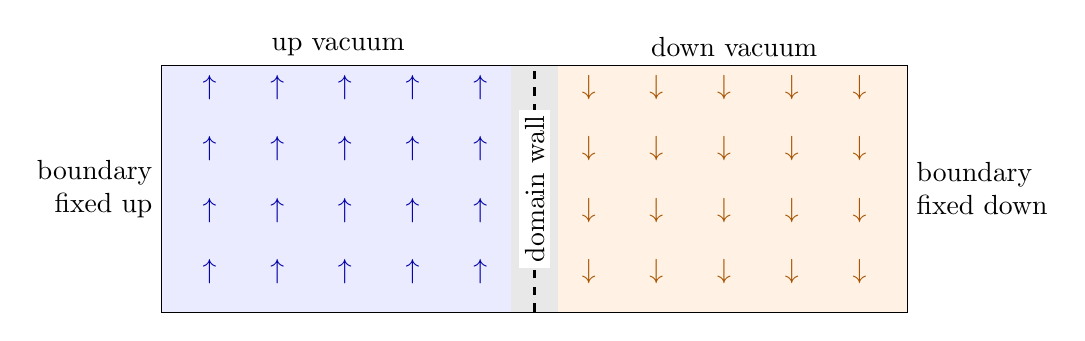
\begin{tikzpicture}[x=0.86cm,y=0.78cm]
  \draw[thick] (0,0) rectangle (11,4);
  \fill[blue!8] (0,0) rectangle (5.15,4);
  \fill[orange!10] (5.85,0) rectangle (11,4);
  \fill[gray!18] (5.15,0) rectangle (5.85,4);
  \foreach \x in {0.7,1.7,2.7,3.7,4.7}
    \foreach \y in {0.65,1.65,2.65,3.65}
      \node[blue!65!black] at (\x,\y) {$\uparrow$};
  \foreach \x in {6.3,7.3,8.3,9.3,10.3}
    \foreach \y in {0.65,1.65,2.65,3.65}
      \node[orange!65!black] at (\x,\y) {$\downarrow$};
  \draw[dashed,thick] (5.5,0) -- (5.5,4);
  \node[above] at (2.6,4) {up vacuum};
  \node[above] at (8.45,4) {down vacuum};
  \node[rotate=90,fill=white,inner sep=2pt] at (5.5,2) {domain wall};
  \node[left,align=right] at (0,2) {boundary\\fixed up};
  \node[right,align=left] at (11,2) {boundary\\fixed down};
\end{tikzpicture}
\end{adjustbox}
\caption{La prueba de contorno para la ruptura espontánea de una simetría discreta. Ambas orientaciones del volumen tienen la misma energía, así que una pared puede separar dominios macroscópicos.}
\end{figure}

\begin{classroomqa}
\audiencequestion{¿El argumento requiere interacciones solo entre vecinos más próximos?\lecturetimestamp{00:18:18}}
\lecturerresponse{No. Una interacción entre segundos vecinos que también favorezca la alineación cambia los detalles, pero no la conclusión. El comportamiento se vuelve más interesante si compiten distintos alcances---por ejemplo, si los vecinos más próximos prefieren alinearse y los siguientes prefieren desalinearse. Eso produce frustración y fases ordenadas más complejas, pero no altera la distinción básica que estamos estableciendo aquí.}
\end{classroomqa}

\begin{classroomqa}
\audiencequestion{¿\emph{Espontánea} se refiere a la gran derivada dentro de la pared?\lecturetimestamp{00:19:05}}
\lecturerresponse{No. Se refiere a que la energía subyacente no favorece la orientación hacia arriba--ni hacia abajo, mientras que el estado fundamental elegido sí lo hace. La respuesta drástica a una perturbación arbitrariamente pequeña revela una inestabilidad. El gradiente solo indica cuánto cuesta la interfaz.}
\end{classroomqa}

\begin{classroomqa}
\audiencequestion{¿El material ya estaba en uno de los dos estados, o se desconocía inicialmente su estado?\lecturetimestamp{00:19:40}}
\lecturerresponse{Depende de su historia. A alta temperatura, el movimiento térmico puede mantener mezclados los espines orientados hacia arriba y hacia abajo, con una magnetización media casi nula. Al enfriarse el material, distintas regiones eligen orientaciones diferentes, se forman paredes de dominio y los dominios crecen. El azar y las pequeñas perturbaciones ambientales determinan qué vacío termina ocupando la mayor parte de la muestra.}
\end{classroomqa}

\section{El mismo argumento en la teoría de campos escalares}

Sustituyamos los espines por un campo escalar real \(\phi(\bm{x},t)\). Fijemos de una vez por todas las convenciones de métrica y normalización, y escribamos
\begin{equation}
\begin{aligned}
  \mathcal L
  &=\frac12\,\partial_\mu\phi\,\partial^\mu\phi-V(\phi),
  \\
  \mathcal E
  &=\frac12\dot\phi^{\,2}+\frac12(\nabla\phi)^2+V(\phi).
\end{aligned}
  \label{eq:l07-real-scalar}
\end{equation}
La notación relativista abreviada de \(\mathcal L\) contiene un término positivo con la derivada temporal y un término negativo con el gradiente espacial; la densidad de energía hamiltoniana tiene positivas ambas contribuciones.

Elijamos un potencial par con dos mínimos degenerados,
\begin{equation}
  V(\phi)=\frac{\lambda}{4}\left(\phi^2-f^2\right)^2,
  \qquad \lambda>0.
  \label{eq:l07-double-well}
\end{equation}
El lagrangiano es invariante bajo \(\phi\mapsto-\phi\), mientras que cualquiera de los dos vacíos uniformes
\begin{equation}
  \phi(\bm{x})=+f,
  \qquad\hbox{or}\qquad
  \phi(\bm{x})=-f
\end{equation}
elige uno de los lados. En cambio, un potencial con un único mínimo en \(\phi=0\) tiene un vacío simétrico y no presenta ruptura espontánea de la simetría.

Fijemos \(\phi=+f\) en un lado de la muestra y \(\phi=-f\) en el otro. El campo no puede saltar sin costo, porque
\begin{equation}
  E_{\rm wall}
  =\int dx\left[
      \frac12\left(\frac{d\phi}{dx}\right)^2+V(\phi)-V(f)
    \right].
  \label{eq:l07-wall-energy}
\end{equation}
Un salto abrupto hace que \(d\phi/dx\) sea enorme. Por tanto, la pared de energía mínima distribuye el cambio en una anchura finita, equilibrando la energía del gradiente con el costo potencial de pasar de un mínimo al otro. La conocida solución tipo kink para el potencial de la Ec.~\eqref{eq:l07-double-well} es
\begin{equation}
  \phi_{\rm wall}(x)
  =f\tanh\!\left[f\sqrt{\frac{\lambda}{2}}\,(x-x_0)\right],
  \label{eq:l07-kink}
\end{equation}
una realización explícita de la transición suave descrita en la pizarra.
\editorialnote{El argumento de la lección se basa en la forma del potencial y en el término de gradiente, pero no resuelve la ecuación de campo. La ecuación \eqref{eq:l07-kink} se incluye como solución estándar del modelo indicado, para concretar cualitativamente la pared sin alterar el argumento.}

Incline ligeramente el doble pozo y uno de los mínimos quedará más bajo. El propio lagrangiano será entonces asimétrico. Aún puede aparecer temporalmente una pared, pero el falso vacío, de mayor energía, ejerce presión sobre ella; la pared se mueve y la fase favorecida se expande. Esta es la versión de la teoría de campos de la ruptura explícita causada por un campo magnético externo.

Hasta ahora, la simetría ha sido discreta. La física de partículas está dominada por grupos continuos como \(U(1)\), \(SU(2)\) y \(SU(3)\). Una simetría continua cambia la historia de los defectos e introduce un nuevo tipo de partícula.

\section{Un campo complejo y la simetría global \texorpdfstring{\(U(1)\)}{U(1)}}

\subsection{Rotaciones en un plano interno}

Sea
\begin{equation}
  \phi=\phi_R+i\phi_I,
  \qquad
  \phi^*=\phi_R-i\phi_I,
  \qquad
  \phi^*\phi=\phi_R^2+\phi_I^2.
  \label{eq:l07-components}
\end{equation}
Los ejes \(\phi_R\) y \(\phi_I\) forman un espacio interno de campos, no dos direcciones del espacio ordinario. Un escalar complejo no es más que dos campos escalares reales reunidos de manera que las rotaciones en este plano interno queden manifiestas.

\begin{figure}[htbp]
\centering
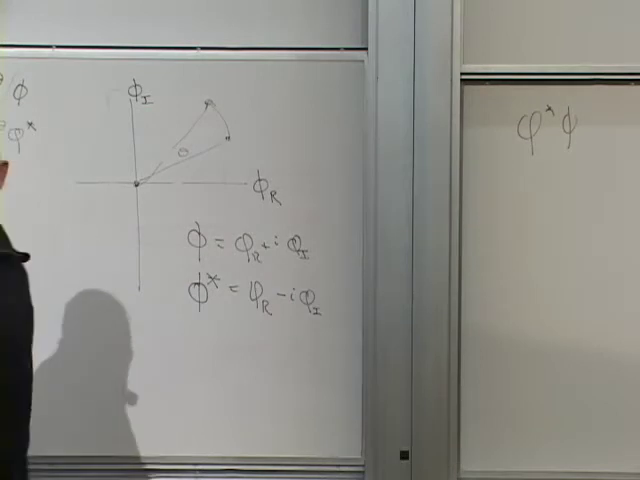
\includegraphics[width=0.80\textwidth]{lecture_07_figure_02.png}
\caption{El campo complejo en el plano interno \((\phi_R,\phi_I)\). La pizarra muestra la descomposición de \(\phi\) y \(\phi^*\), y el radio invariante \(\phi^*\phi\).}
\lectureframe{00:33:33}
\end{figure}

Tomemos el lagrangiano
\begin{equation}
  \mathcal L
  =\partial_\mu\phi^*\,\partial^\mu\phi
   -V(\phi^*\phi).
  \label{eq:l07-complex-lagrangian}
\end{equation}
Para un campo complejo se omite el factor convencional \(1/2\), porque este único producto ya contiene los términos cinéticos de ambas componentes reales. La transformación
\begin{equation}
  \phi'(x)=e^{i\theta}\phi(x),
  \qquad
  \phi^{*\prime}(x)=e^{-i\theta}\phi^*(x)
  \label{eq:l07-global-u1}
\end{equation}
rota por el mismo ángulo todos los valores del campo. Aquí \(\theta\) es constante en el espacio y el tiempo. La prima indica el campo transformado; no es una derivada.

Como \(\theta\) es constante,
\begin{equation}
  \partial_\mu\phi'=e^{i\theta}\partial_\mu\phi,
  \qquad
  \partial_\mu\phi^{*\prime}
  =e^{-i\theta}\partial_\mu\phi^*.
\end{equation}
Las fases se cancelan en el término cinético, y
\(\phi^{*\prime}\phi'=\phi^*\phi\). Así, todo potencial que dependa únicamente de \(\phi^*\phi\) tiene la misma simetría. Un término que dependiera solo de \(\phi_R\) seleccionaría una dirección en el plano interno y la rompería explícitamente.

\subsection{Un mínimo puntual y un círculo de mínimos}

Hay dos tipos cualitativamente distintos de potenciales simétricos. El primero tiene su único mínimo en el origen; por ejemplo,
\begin{equation}
  V_{\rm unbroken}=m^2\phi^*\phi,
  \qquad m^2>0.
\end{equation}
Su gráfica es un paraboloide con simetría rotacional. El vacío \(\phi=0\) permanece fijo bajo toda rotación, así que la simetría no está rota.

Elijamos ahora
\begin{equation}
  V_{\rm broken}
  =-a\,\phi^*\phi+b(\phi^*\phi)^2,
  \qquad a,b>0.
  \label{eq:l07-mexican-hat}
\end{equation}
El término cuadrático negativo empuja el campo para alejarlo del origen, mientras que el término cuártico positivo impide que se dispare hasta el infinito. Si escribimos \(r^2=\phi^*\phi\), la minimización da
\begin{equation}
  \frac{dV}{d(r^2)}=-a+2br^2=0,
  \qquad
  r^2=f^2=\frac{a}{2b}.
  \label{eq:l07-vacuum-radius}
\end{equation}
Por tanto, los mínimos forman un círculo. El potencial tiene simetría rotacional perfecta, pero un estado fundamental uniforme debe elegir un punto de ese círculo.

\begin{figure}[htbp]
\centering
\includegraphics[width=0.72\textwidth]{lecture_07_figure_06.png}
\caption{El potencial que rompe la simetría, dibujado como una superficie de revolución. El origen es inestable y los mínimos degenerados forman el fondo circular.}
\lectureframe{00:37:25}
\end{figure}

Imaginemos que en cada punto del espacio ordinario el campo es una pequeña flecha en este plano interno. El potencial exige que cada flecha tenga longitud \(f\). La energía del gradiente exige que las flechas cercanas apunten casi en la misma dirección. En consecuencia, el estado fundamental tiene el mismo ángulo en todas partes, pero la ley no prefiere ninguno. Eso es la ruptura espontánea de una simetría continua.

\section{De una pared de dominio a un giro suave}

Repitamos el experimento con los contornos. En el contorno izquierdo fijemos el campo en un punto de vacío \(A\); en el derecho, en otro punto de vacío \(B\). Un salto localizado haría que el gradiente fuera grande. Sin embargo, a diferencia del caso discreto, el campo puede permanecer en el fondo del potencial mientras cambia continuamente alrededor del círculo.

A baja energía, escribamos el campo como \(\phi=f e^{i\alpha(x)}\). En una dimensión espacial, la energía relevante es
\begin{equation}
  E[\alpha]
  =f^2\int_0^L dx\,\left(\frac{d\alpha}{dx}\right)^2.
  \label{eq:l07-angle-functional}
\end{equation}
Para ángulos extremos fijos, la variación da
\begin{equation}
  \frac{d^2\alpha}{dx^2}=0,
  \qquad
  \alpha(x)=\alpha_A+
    \frac{\alpha_B-\alpha_A}{L}\,x.
  \label{eq:l07-linear-twist}
\end{equation}
La configuración preferida distribuye el giro uniformemente por toda la muestra. Su energía escala como
\begin{equation}
  E_{\rm twist}
  =f^2\frac{(\alpha_B-\alpha_A)^2}{L},
  \label{eq:l07-twist-energy}
\end{equation}
por lo que puede hacerse arbitrariamente pequeña al aumentar \(L\).

\begin{figure}[htbp]
\centering
\begin{adjustbox}{max width=\linewidth}
\begin{tikzpicture}[x=0.95cm,y=0.95cm]
  \begin{scope}
    \draw[->] (0,0) -- (6.2,0) node[right] {$x$};
    \draw[->] (0,0) -- (0,3.5) node[above] {$\alpha(x)$};
    \draw[very thick,blue!70!black] (0.45,0.65) -- (5.7,2.85);
    \fill (0.45,0.65) circle (1.8pt) node[left] {$\alpha_A$};
    \fill (5.7,2.85) circle (1.8pt) node[right] {$\alpha_B$};
    \node at (3.1,-0.65) {physical space};
  \end{scope}
  \begin{scope}[xshift=9.2cm,yshift=1.65cm]
    \draw[thick] (0,0) circle (1.8);
    \fill (1.55,-0.92) circle (1.8pt) node[below right] {$A$};
    \fill (-0.45,1.74) circle (1.8pt) node[above] {$B$};
    \draw[very thick,blue!70!black,-{Latex[length=2.5mm]}]
      (1.55,-0.92) arc[start angle=-31,end angle=104,radius=1.8];
    \node at (0,-2.35) {vacuum circle};
  \end{scope}
\end{tikzpicture}
\end{adjustbox}
\caption{La misma configuración de baja energía en dos descripciones. El ángulo varía linealmente a través del espacio físico, mientras que el campo sigue el arco corto del círculo de vacío en el espacio interno.}
\end{figure}

\begin{classroomqa}
\audiencequestion{Hay dos maneras de recorrer el círculo. ¿Qué camino sigue el campo y puede quedar atrapado en el más largo?
\lecturetimestamp{00:41:54}}
\lecturerresponse{Para extremos genéricos, la ruta angular más corta tiene un gradiente menor y, por tanto, menor energía. Si los extremos son diametralmente opuestos, las dos rutas más sencillas son degeneradas. Una configuración preparada moviendo lentamente uno de los extremos puede conservar un número de vueltas adicional y quedar atrapada tras una barrera de energía; pero, para un par determinado de extremos ordinarios, la ruta más corta sin torsión es el estado fundamental.}
\end{classroomqa}

\begin{classroomqa}
\audiencequestion{¿Podría el camino salir del fondo del valle y atravesar el interior, acortándose en conjunto?
\lecturetimestamp{00:43:32}}
\lecturerresponse{En el régimen de baja energía y muestras largas, no compensa subir por el potencial radial. Mantener el radio en su valor de vacío y variar el ángulo linealmente minimiza la energía efectiva, como muestra el cálculo variacional anterior. En un sistema finito con un potencial específico se pueden minimizar conjuntamente el movimiento radial y el angular, pero la conclusión de Goldstone se refiere al límite de longitudes de onda arbitrariamente grandes, en el que prevalece el movimiento suave a lo largo del valle.}
\end{classroomqa}

\begin{classroomqa}
\audiencequestion{¿Qué cambia si se inclina el valle circular para que un ángulo tenga menor energía?
\lecturetimestamp{00:44:33}}
\lecturerresponse{Entonces la simetría se rompe explícitamente. Un punto se convierte en el verdadero estado fundamental, el movimiento a lo largo del círculo adquiere una fuerza restauradora y la excitación angular deja de ser exactamente sin masa.}
\end{classroomqa}

\section{La masa como costo de una oscilación con momento nulo}

El giro suave revela un campo cuya energía procede únicamente de los gradientes. Para entender por qué eso implica una partícula sin masa, comparemos la relación de dispersión relativista
\begin{equation}
  \omega^2=\bm{k}^2+m^2.
  \label{eq:l07-dispersion}
\end{equation}
Una onda \(e^{i(\bm{k}\cdot\bm{x}-\omega t)}\) lleva momento \(\bm{k}\).
Si \(m=0\), su energía tiende a cero cuando la longitud de onda tiende al infinito:
\(\omega=|\bm{k}|\to0\). Si \(m\ne0\), un modo espacialmente homogéneo \(\bm{k}=0\) sigue oscilando con frecuencia \(\omega=m\). La masa es la energía irreducible con momento nulo.

Esta misma distinción se observa en el lagrangiano. Un término
\begin{equation}
  -\frac12m^2\varphi^2
\end{equation}
aporta una fuerza restauradora incluso para un desplazamiento homogéneo. Un campo que solo tiene términos con derivadas carece de esa fuerza restauradora: al aumentar la longitud de onda, su energía de gradiente se aproxima a cero.

\subsection{Las variables polares separan los dos modos}

Escribamos el campo complejo con simetría rota como
\begin{equation}
  \phi(x)=\rho(x)e^{i\alpha(x)}.
  \label{eq:l07-polar}
\end{equation}
Tanto \(\rho\) como \(\alpha\) son campos. Al derivar se obtiene
\begin{align}
  \partial_\mu\phi
  &=e^{i\alpha}
    \left(\partial_\mu\rho+i\rho\,\partial_\mu\alpha\right),\\
  \partial_\mu\phi^*
  &=e^{-i\alpha}
    \left(\partial_\mu\rho-i\rho\,\partial_\mu\alpha\right).
\end{align}
Los términos cruzados se cancelan y queda
\begin{equation}
  \partial_\mu\phi^*\,\partial^\mu\phi
  =(\partial_\mu\rho)(\partial^\mu\rho)
   +\rho^2(\partial_\mu\alpha)(\partial^\mu\alpha).
  \label{eq:l07-polar-kinetic}
\end{equation}
Como \(\phi^*\phi=\rho^2\),
\begin{equation}
  \mathcal L
  =(\partial\rho)^2+\rho^2(\partial\alpha)^2-V(\rho^2).
  \label{eq:l07-polar-lagrangian}
\end{equation}
El potencial contiene \(\rho\), pero no \(\alpha\). Esa ausencia expresa la simetría en su forma más útil.

\begin{figure}[htbp]
\centering
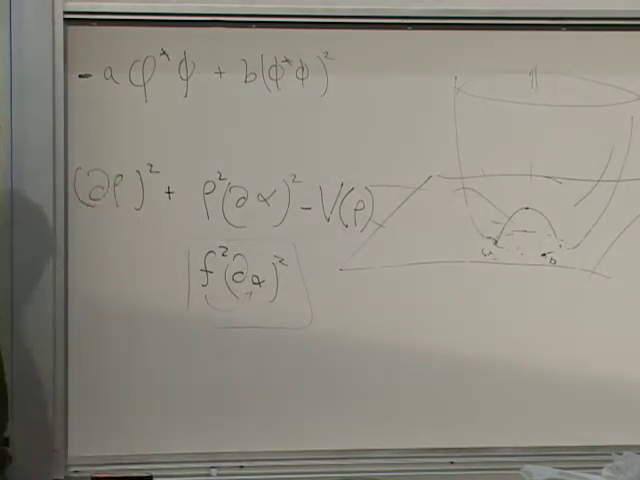
\includegraphics[width=0.88\textwidth]{lecture_07_figure_03.png}
\caption{El lagrangiano en variables polares, su término angular de baja energía enmarcado y el potencial que rompe la simetría. El movimiento radial hace subir por el potencial; el angular sigue el valle.}
\lectureframe{00:56:40}
\end{figure}

Para una excitación de energía muy baja, el campo permanece cerca de \(\rho=f\). Entonces
\begin{equation}
  \mathcal L_{\rm angular}
  \simeq f^2(\partial_\mu\alpha)(\partial^\mu\alpha).
\end{equation}
Definamos el campo angular con normalización canónica, salvo la convención para los factores de \(1/2\), mediante
\begin{equation}
  \beta=\sqrt{2}\,f\alpha,
  \qquad
  \mathcal L_{\rm angular}
  =\frac12(\partial_\mu\beta)(\partial^\mu\beta).
  \label{eq:l07-goldstone-field}
\end{equation}
No hay término \(\beta^2\). Los cuantos de este campo angular no tienen masa. Son los bosones de Goldstone.

El campo radial se comporta de otra manera. Si desplazamos \(\rho\) de \(f\) en todas partes a la vez, rueda de vuelta, sobrepasa el mínimo y oscila alrededor del fondo del valle. Si \(\rho=f+h\), el desarrollo de la Ec.~\eqref{eq:l07-mexican-hat} produce
\begin{equation}
  V(f+h)=V(f)+\frac12m_h^2h^2+\cdots,
\end{equation}
por lo que \(h\) tiene masa. Geométricamente, la dirección angular es plana y la radial es curva.

\begin{classroomqa}
\audiencequestion{Si el campo se desplaza radialmente, ¿simplemente vuelve a bajar? ¿Qué ocurre después?\lecturetimestamp{00:57:10}}
\lecturerresponse{Sin movimiento angular, cae hacia el mínimo, lo sobrepasa y oscila radialmente. Una oscilación homogénea tiene momento espacial nulo, pero frecuencia distinta de cero; esa frecuencia es la masa de la excitación radial. En cambio, un desplazamiento angular homogéneo termina en otro vacío y no tiene fuerza restauradora.}
\end{classroomqa}

Este es el contenido del principio de Goldstone en el ejemplo actual: la ruptura espontánea de una simetría global continua produce un modo sin masa por cada dirección plana independiente de la variedad de vacíos.
\editorialnote{El enunciado supone las condiciones habituales de la teoría relativista de campos. En sistemas de muchos cuerpos no relativistas, el recuento y la dispersión de los modos de Nambu--Goldstone pueden ser más sutiles, pero la conclusión de la lección sobre longitudes de onda largas sigue siendo válida para este modelo relativista \(U(1)\).}

\section{Ondas de espín, cuerdas y sonido}

El teorema es abstracto, pero su mecanismo resulta familiar. En un ferromagneto isotrópico, se pueden rotar todos los espines juntos sin cambiar la energía. Si la orientación varía muy lentamente a través de la muestra, se obtiene una onda de espín. Su costo se anula al tender a cero el número de onda, así que es el modo de Goldstone de la simetría rota por rotaciones de espín.

Una cuerda elástica larga ofrece otra imagen. Ignorando la gravedad, montemos los extremos de modo que se pueda trasladar verticalmente toda la cuerda. Una traslación vertical uniforme no cuesta energía. Si hacemos que la traslación varíe lentamente a lo largo de la cuerda, se convierte en una onda transversal de longitud de onda larga. La operación de simetría uniforme se ha convertido en una deformación suave que depende de la posición.

\begin{figure}[htbp]
\centering
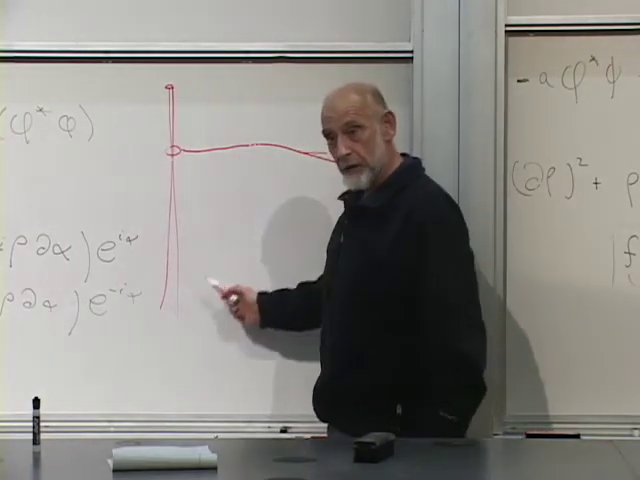
\includegraphics[width=0.68\textwidth]{lecture_07_figure_04.png}
\caption{El perfil de la cuerda que varía lentamente, dibujado durante la analogía con el modo de Goldstone. Lo importante físicamente es la pequeña pendiente de una deformación de longitud de onda larga, no la posición vertical de la curva.}
\lectureframe{01:04:19}
\end{figure}

\begin{classroomqa}
\audiencequestion{¿Puede la cuerda transportar energía de oscilación y tener momento nulo?
\lecturetimestamp{01:04:41}}
\lecturerresponse{Hay que distinguir el momento mecánico vertical del momento de onda a lo largo de la cuerda. Una onda estacionaria puede tener momento neto nulo porque es una superposición de modos con \(+k\) y \(-k\), y aun así transportar energía. En la analogía con la teoría de campos, el momento se refiere al número de onda a lo largo del eje; el desplazamiento vertical representa la coordenada interna del campo.}
\end{classroomqa}

Un muelle extensible ilustra la versión longitudinal. Traslademos todo el muelle infinito idealizado a lo largo de su eje: nada cambia. Si trasladamos las partes vecinas en cantidades ligeramente distintas, el resultado es una onda de compresión suave. En un sólido o un fluido, el sonido de longitud de onda larga surge de desplazamientos colectivos y variaciones de densidad. Las ondas de espín, las ondas transversales en una cuerda y el sonido no son la misma excitación microscópica, pero comparten el patrón decisivo: una operación continua uniforme no cuesta energía, y su versión que varía lentamente se convierte en un modo blando.
\editorialnote{En un cristal, los fonones acústicos se describen convencionalmente como modos de Nambu--Goldstone asociados a la ruptura espontánea de las traslaciones continuas. La cuerda y el muelle extensible son analogías mecánicas que se usan en la lección para mostrar la misma estructura de energía que depende únicamente de derivadas.}

La terminología merece una breve broma de clase: son bosones de \emph{Goldstone}, llamados así por Jeffrey Goldstone, no bosones gauge. La lección señala que Goldstone era amigo de Susskind y luego pasa al tema realmente distinto de la invariancia gauge.

\section{De la simetría global de fase a la simetría gauge}

La simetría de fase \(U(1)\) ya apareció en el curso como la simetría asociada a la conservación de la carga. Los campos de partículas cargadas son complejos, y multiplicarlos por una fase común deja inalterada la teoría global. Se puede hablar de carga eléctrica para facilitar la intuición, aunque la carga podría representar otro número cuántico \(U(1)\). El fotón real no tiene masa; el objetivo final es un campo similar al fotón, como el \(Z\) masivo.

La nueva pregunta es si
\begin{equation}
  \phi'(x)=e^{i\theta(x)}\phi(x)
  \label{eq:l07-local-u1}
\end{equation}
puede ser una simetría cuando \(\theta\) varía arbitrariamente por el espacio-tiempo. La función \(\theta(x)\) es un parámetro de transformación, no un campo dinámico adicional. Comprobemos la propuesta derivando:
\begin{equation}
  \partial_\mu\phi'
  =e^{i\theta}
   \left[\partial_\mu\phi+i(\partial_\mu\theta)\phi\right].
  \label{eq:l07-local-derivative}
\end{equation}
El término adicional no aparecía cuando \(\theta\) era constante. Para el conjugado,
\begin{equation}
  \partial_\mu\phi^{*\prime}
  =e^{-i\theta}
   \left[\partial_\mu\phi^*-i(\partial_\mu\theta)\phi^*\right].
\end{equation}
El producto es
\begin{align}
  \partial_\mu\phi^{*\prime}\partial^\mu\phi'
  ={}&
  \partial_\mu\phi^*\partial^\mu\phi
  i\left(
      \phi\,\partial_\mu\phi^*
      -\phi^*\partial_\mu\phi
    \right)\partial^\mu\theta
  \nonumber\\
  &+\phi^*\phi\,
    \partial_\mu\theta\,\partial^\mu\theta.
  \label{eq:l07-local-failure}
\end{align}
El potencial sigue siendo invariante porque también lo es \(\phi^*\phi\), pero el término cinético ordinario no lo es. Una simetría global no se convierte automáticamente en una simetría local.

\begin{classroomqa}
\audiencequestion{En la imagen del sombrero mexicano, ¿este fallo significa que hay bultos alrededor del valle circular?
\lecturetimestamp{01:19:37}}
\lecturerresponse{No. El potencial puede seguir siendo perfectamente plano en la dirección angular. El costo adicional proviene de los gradientes cuando la fase difiere entre distintos puntos del espacio-tiempo. No se trata de ondulaciones del valle: es el término ordinario de derivadas que detecta la variación espacial.}
\end{classroomqa}

\subsection{El campo vectorial compensador}

Las interacciones del fotón de la naturaleza, \(W\), \(Z\) y los gluones están organizadas por simetrías gauge locales, no solo por transformaciones rígidas. Para que la operación de fase local sea una simetría, ampliemos la teoría con un campo de cuatro vectores \(A_\mu\). En electromagnetismo, \(A_0\) es el potencial escalar y las tres componentes espaciales forman el potencial vector. Sus derivadas construyen los campos eléctrico y magnético.

Elijamos una convención internamente consistente:
\begin{equation}
  \phi'=e^{i\theta}\phi,
  \qquad
  A'_\mu=A_\mu-\partial_\mu\theta,
  \qquad
  D_\mu=\partial_\mu+iA_\mu.
  \label{eq:l07-gauge-convention}
\end{equation}
Al comprobar la cancelación, en la pizarra se cambia un signo; la Ec.
\eqref{eq:l07-gauge-convention}
fija conjuntamente los tres signos. Por ahora, las constantes de acoplamiento y de carga se han absorbido en \(A_\mu\).
\editorialnote{Con la carga explícita \(q\) y el acoplamiento \(g\), se puede escribir \(D_\mu=\partial_\mu+igqA_\mu\) y
\(A'_\mu=A_\mu-(gq)^{-1}\partial_\mu\theta\). La lección omite estas constantes para que la cancelación quede a la vista.}

Para el campo conjugado,
\begin{equation}
  D_\mu\phi^*=\partial_\mu\phi^*-iA_\mu\phi^*.
\end{equation}
Ahora bien,
\begin{align}
  D'_\mu\phi'
  &=
  \left(\partial_\mu+iA'_\mu\right)e^{i\theta}\phi
  \nonumber\\
  &=
  e^{i\theta}
  \left[
    \partial_\mu\phi+i(\partial_\mu\theta)\phi
    +i(A_\mu-\partial_\mu\theta)\phi
  \right]
  \nonumber\\
  &=e^{i\theta}D_\mu\phi.
  \label{eq:l07-covariant-transform}
\end{align}
La transformación de \(A_\mu\) cancela la derivada no deseada de \(\theta\). Asimismo,
\begin{equation}
  D'_\mu\phi^{*\prime}=e^{-i\theta}D_\mu\phi^*.
\end{equation}
Su producto es invariante. El adjetivo \emph{covariante} significa que la derivada se transforma de la misma manera sencilla que el propio campo.

\section{Dinámica del campo gauge}

Introducir \(A_\mu\) solo para reparar una derivada lo dejaría sin dinámica propia. El tensor de campo gauge invariante es
\begin{equation}
  F_{\mu\nu}
  =\partial_\mu A_\nu-\partial_\nu A_\mu.
  \label{eq:l07-field-strength}
\end{equation}
Es antisimétrico, por lo que \(F_{\mu\mu}=0\). Sus componentes tiempo--espacio contienen el campo eléctrico, mientras que sus componentes espacio--espacio contienen el campo magnético. En el lenguaje familiar de los vectores tridimensionales, la densidad de energía electromagnética es proporcional a \(\bm E^2+\bm B^2\), mientras que el lagrangiano lorentziano es proporcional a \(\bm E^2-\bm B^2\), con signos que dependen de la convención de métrica.

\begin{classroomqa}
\audiencequestion{¿Cuáles son la energía y el lagrangiano del campo electromagnético?\lecturetimestamp{01:33:20}}
\lecturerresponse{La energía se construye a partir de \(E^2+B^2\); el lagrangiano usa \(E^2-B^2\). En forma covariante, este último se escribe como un múltiplo convencional de \(F_{\mu\nu}F^{\mu\nu}\). El tensor antisimétrico es el rotacional cuatridimensional del potencial vector.}
\end{classroomqa}

El tensor de campo es invariante gauge por sí mismo:
\begin{align}
  F'_{\mu\nu}
  &=
  \partial_\mu(A_\nu-\partial_\nu\theta)
  -\partial_\nu(A_\mu-\partial_\mu\theta)
  \nonumber\\
  &=
  F_{\mu\nu}
  -\partial_\mu\partial_\nu\theta
  +\partial_\nu\partial_\mu\theta
  =F_{\mu\nu}.
  \label{eq:l07-field-strength-invariant}
\end{align}
La igualdad final se sigue de que las derivadas parciales mixtas ordinarias conmutan. Por tanto, un lagrangiano gauge invariante estándar es
\begin{equation}
  \boxed{
  \mathcal L
  =(D_\mu\phi)^*D^\mu\phi
  -V(\phi^*\phi)
  -\frac14F_{\mu\nu}F^{\mu\nu}}
  \label{eq:l07-scalar-qed}
\end{equation}
hasta el signo y la normalización elegidos para la métrica.

\begin{figure}[htbp]
\centering
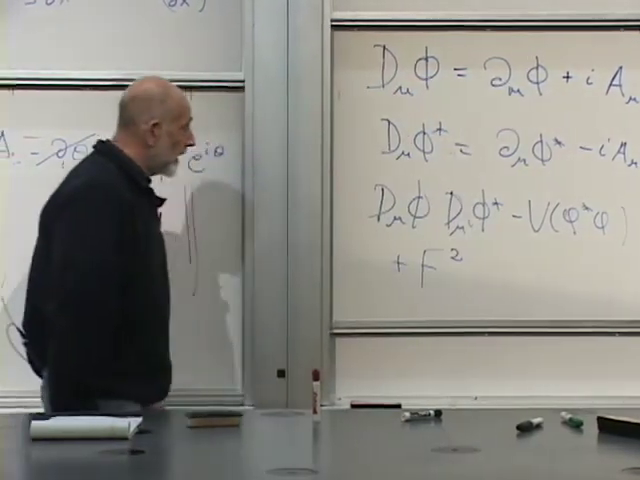
\includegraphics[width=0.84\textwidth]{lecture_07_figure_05.png}
\caption{Las derivadas covariantes y el lagrangiano gauge invariante completo, tal como aparecen en la pizarra. Allí se omiten los factores numéricos para que la estructura de las transformaciones siga siendo visible.}
\lectureframe{01:38:45}
\end{figure}

Esta construcción convierte una simetría global \(U(1)\) en una local, pero lo hace a costa---o, físicamente, a cambio---de introducir un nuevo campo vectorial. En el ejemplo abeliano, ese campo es el potencial electromagnético.

\begin{classroomqa}
\audiencequestion{El lagrangiano con el que empezamos usaba derivadas ordinarias. ¿Por qué podemos sustituirlas por derivadas covariantes y llamar al resultado la teoría real?\lecturetimestamp{01:42:55}}
\lecturerresponse{Estamos construyendo una teoría distinta y ampliada: materia cargada más un campo gauge. La invariancia gauge local determina su acoplamiento. La teoría cuántica resultante es una estructura matemática coherente y concuerda con la manera en que la naturaleza organiza los campos gauge del fotón y de la interacción débil. Acoplar sin coherencia un campo vectorial relativista puede introducir polarizaciones no físicas y violaciones de la probabilidad, así que el principio gauge no es una mera reformulación cosmética de la antigua teoría escalar libre.}
\end{classroomqa}

\begin{classroomqa}
\audiencequestion{Así que añadir el nuevo campo es la justificación esencial de la modificación?\lecturetimestamp{01:44:57}}
\lecturerresponse{Sí. Sin \(A_\mu\), la derivada de un campo rotado localmente contiene un término \(\partial_\mu\theta\) que no se cancela. Con \(A_\mu\) y su ley de transformación, la cancelación funciona. En lenguaje geométrico, \(A_\mu\) es una conexión en un fibrado; esas matemáticas más profundas son reales y útiles, pero el álgebra anterior contiene lo necesario aquí.}
\end{classroomqa}

\section{Por qué está prohibida una masa desnuda para un bosón gauge}

Para un campo bosónico ordinario, la masa se representa mediante un término cuadrático. Resulta tentador añadir
\begin{equation}
  \Delta\mathcal L_{\rm Proca}
  =\frac12m^2A_\mu A^\mu.
  \label{eq:l07-proca}
\end{equation}
Pero bajo \(A_\mu\mapsto A_\mu-\partial_\mu\theta\),
\begin{equation}
  A'_\mu A^{\mu\prime}
  =
  A_\mu A^\mu
  -2A^\mu\partial_\mu\theta
  +\partial_\mu\theta\,\partial^\mu\theta,
\end{equation}
por lo que la ecuación~\eqref{eq:l07-proca} no es invariante gauge. No podemos introducir a mano una masa en esta teoría gauge y conservar al mismo tiempo su simetría local.

\begin{figure}[htbp]
\centering
\includegraphics[width=0.72\textwidth]{lecture_07_figure_07.png}
\caption{La masa vectorial desnuda propuesta
\(\tfrac12m^2A_\mu A^\mu\). Su falta de invariancia bajo
\(A_\mu\mapsto A_\mu-\partial_\mu\theta\) es el obstáculo que prepara el terreno para el mecanismo de Higgs.}
\lectureframe{01:39:48}
\end{figure}

Este es el aparente callejón sin salida. La invariancia gauge explica que el fotón no tenga masa y protege la teoría de grados de libertad no físicos, pero \(W\) y \(Z\) tienen masa. La salida no puede consistir en añadir explícitamente una masa vectorial. Debe surgir de los campos que ya están presentes en un lagrangiano invariante gauge.

\begin{classroomqa}
\audiencequestion{¿La introducción de la invariancia gauge produce por sí misma el bosón de Goldstone?\lecturetimestamp{01:45:51}}
\lecturerresponse{No. El bosón de Goldstone surgió cuando se rompió espontáneamente una simetría \emph{global} continua, antes de introducir el potencial vectorial. Una vez que la simetría es local, \(A_\mu\) puede compensar una fase variable. En la teoría gauge rota, el modo angular deja de ser una partícula independiente sin masa; proporciona la polarización adicional del campo vectorial, que ahora tiene masa. En la próxima conferencia deduciremos esta afirmación en lugar de limitarnos a enunciarla.}
\end{classroomqa}

\begin{classroomqa}
\audiencequestion{¿Explica algo de esto por qué los ríos serpentean?
\lecturetimestamp{01:47:03}}
\lecturerresponse{Aquí no se conoce ninguna conexión directa. Los remolinos de los fluidos e incluso las formas de los organismos pueden describirse sin duda mediante métodos de simetría, y nunca debería sorprendernos encontrar ideas de teoría de campos en lugares inesperados, pero en la conferencia no se propone ninguna teoría gauge de los meandros fluviales.}\end{classroomqa}

\section{Dónde termina la conferencia}

Ya tenemos los dos ingredientes prometidos al principio. Una simetría global continua con un círculo de vacíos tiene una dirección angular plana, y su variación lenta es un campo de Goldstone sin masa. Una simetría local requiere una conexión gauge y derivadas covariantes, y prohíbe la masa vectorial directa de la ecuación~\eqref{eq:l07-proca}.

El siguiente paso consiste en usar el potencial roto de la ecuación~\eqref{eq:l07-mexican-hat} dentro de la teoría invariante gauge de la ecuación~\eqref{eq:l07-scalar-qed}. Entonces ocurren dos cosas a la vez: la partícula de Goldstone deja de aparecer como partícula independiente en el espectro físico, y el campo vectorial adquiere masa. En el lenguaje pedagógico habitual, se dice que la simetría gauge se rompe espontáneamente; con mayor precisión, la redundancia gauge permanece mientras la teoría entra en una fase de Higgs con una excitación vectorial masiva.
\editorialnote{Una simetría gauge local es una redundancia de la descripción, no una simetría física ordinaria que actúe entre estados observables distintos. La conferencia emplea la expresión abreviada habitual «ruptura espontánea de la simetría gauge». La afirmación física invariante gauge es la reorganización de los grados de libertad en la fase de Higgs.}

Ese es el fenómeno de Higgs. Todavía no lo hemos llevado a cabo. Esta conferencia ha hecho el trabajo, más difícil pero necesario, de precisar el problema lo suficiente para que la solución, cuando llegue, sea inevitable.
